\documentclass[11pt]{article}
\usepackage[T1]{fontenc}
\usepackage[margin=0.8in]{geometry}
\usepackage{graphicx}
\usepackage{xcolor}
\usepackage{listings}
\usepackage{booktabs}
\usepackage{hyperref}
\definecolor{codeblue}{RGB}{36,83,150}
\definecolor{codestring}{RGB}{145,50,45}
\definecolor{codegreen}{RGB}{45,115,75}
\definecolor{codegray}{RGB}{100,100,100}
\lstdefinestyle{python}{
  language=Python, basicstyle=\ttfamily\small,
  keywordstyle=\color{codeblue}\bfseries, stringstyle=\color{codestring},
  commentstyle=\color{codegreen}\itshape, numberstyle=\scriptsize\color{codegray},
  numbers=left, numbersep=8pt, showstringspaces=false, breaklines=true,
  frame=single, rulecolor=\color{black!20}, columns=fullflexible,
  keepspaces=true, upquote=true, tabsize=4
}
\lstset{style=python}
\hypersetup{colorlinks=true,linkcolor=blue!50!black,urlcolor=blue!50!black}
\title{Payoff-Relevant News in a Multiround Asset Market\\\large EDSL shared-state pilot}
\author{EDSL replication study}
\date{October 11, 2026}

\begin{document}
\maketitle

\begin{abstract}
Three independent 30-period market pilots tested a binding change to terminal
redemption after period 5. Redemption rose from \$14 to \$20 in the positive
arm, fell to \$8 in the negative arm, and remained \$14 in the no-news control.
The period-6 mean forecast moved from about \$14.2 to \$19.41 after positive
news and \$8.83 after negative news; the control stayed at \$14.23. News also
shifted submitted buy and sell limits in the expected direction. No orders
crossed, however, so no shares traded. The pilots show a clear belief and quote
response but do not demonstrate a transaction-price response. This report
documents the experiment and its new state-machine implementation.
\end{abstract}

\section{Design}
Each market has 12 traders, each starting with \$100 cash and four shares.
Cash earns 5\% interest; each share pays a common \$0.40 or \$1.00 dividend
with equal probability. The initial terminal redemption is \$14. Four traders
per market follow each of three payoff-based trading styles: value buyer, value
seller, or flexible value trader. Style, prompts, initial endowments, and model
settings are the same in every condition.

After period 5 settlement and before period 6 orders, the exchange publishes a
binding payoff update to every trader in the positive and negative arms. The
positive message changes redemption to \$20; the negative message changes it
to \$8. The no-news control receives no payoff update and stays at \$14.
Dividends remain unchanged. The three markets share replicate seed 153101, so
the dividend draws are paired across conditions. Treatment is assigned at the
market level because traders share one public tape and their actions spill over.

\section{Pilot results}
\begin{center}
\begin{tabular}{lrrr}
\toprule
Measure & Positive & Negative & Control \\
\midrule
Period 5 mean current-price forecast & \$14.22 & \$14.32 & \$14.23 \\
Period 6 mean current-price forecast & \$19.41 & \$8.83 & \$14.23 \\
Period 5 mean 10-period forecast & \$15.32 & \$15.08 & \$14.89 \\
Period 6 mean 10-period forecast & \$21.54 & \$9.97 & \$14.89 \\
Buy orders & 219 & 195 & 149 \\
Sell orders & 92 & 114 & 120 \\
Holds & 49 & 51 & 91 \\
Shares traded & 0 & 0 & 0 \\
Trading periods & 0 / 30 & 0 / 30 & 0 / 30 \\
Ending cash per trader & \$703.21 & \$655.21 & \$679.21 \\
\bottomrule
\end{tabular}
\end{center}

The post-update change in mean current-price forecast was +\$5.19 in the
positive arm, -\$5.48 in the negative arm, and \$0.00 in control. The period-6
best bid and best ask were \$19.00 and \$21.00 in the positive arm, \$9.50 and
\$10.00 in the negative arm, and \$13.90 and \$15.00 in control. The public
fundamental update therefore moved beliefs and quotes as intended. In all
three markets, the highest buy limit remained below the lowest sell limit, so
no transactions occurred.

The individual submitted buy limits make the change directly visible. Among
the six traders in each arm who submitted buy orders both before and after the
announcement, the mean bid rose by \$3.60 after positive news, fell by \$5.28
after negative news, and changed by \$0.00 in control. Figure~\ref{fig:bids}
connects each trader's own pre- and post-announcement buy limit.

\begin{figure}[ht]
\centering
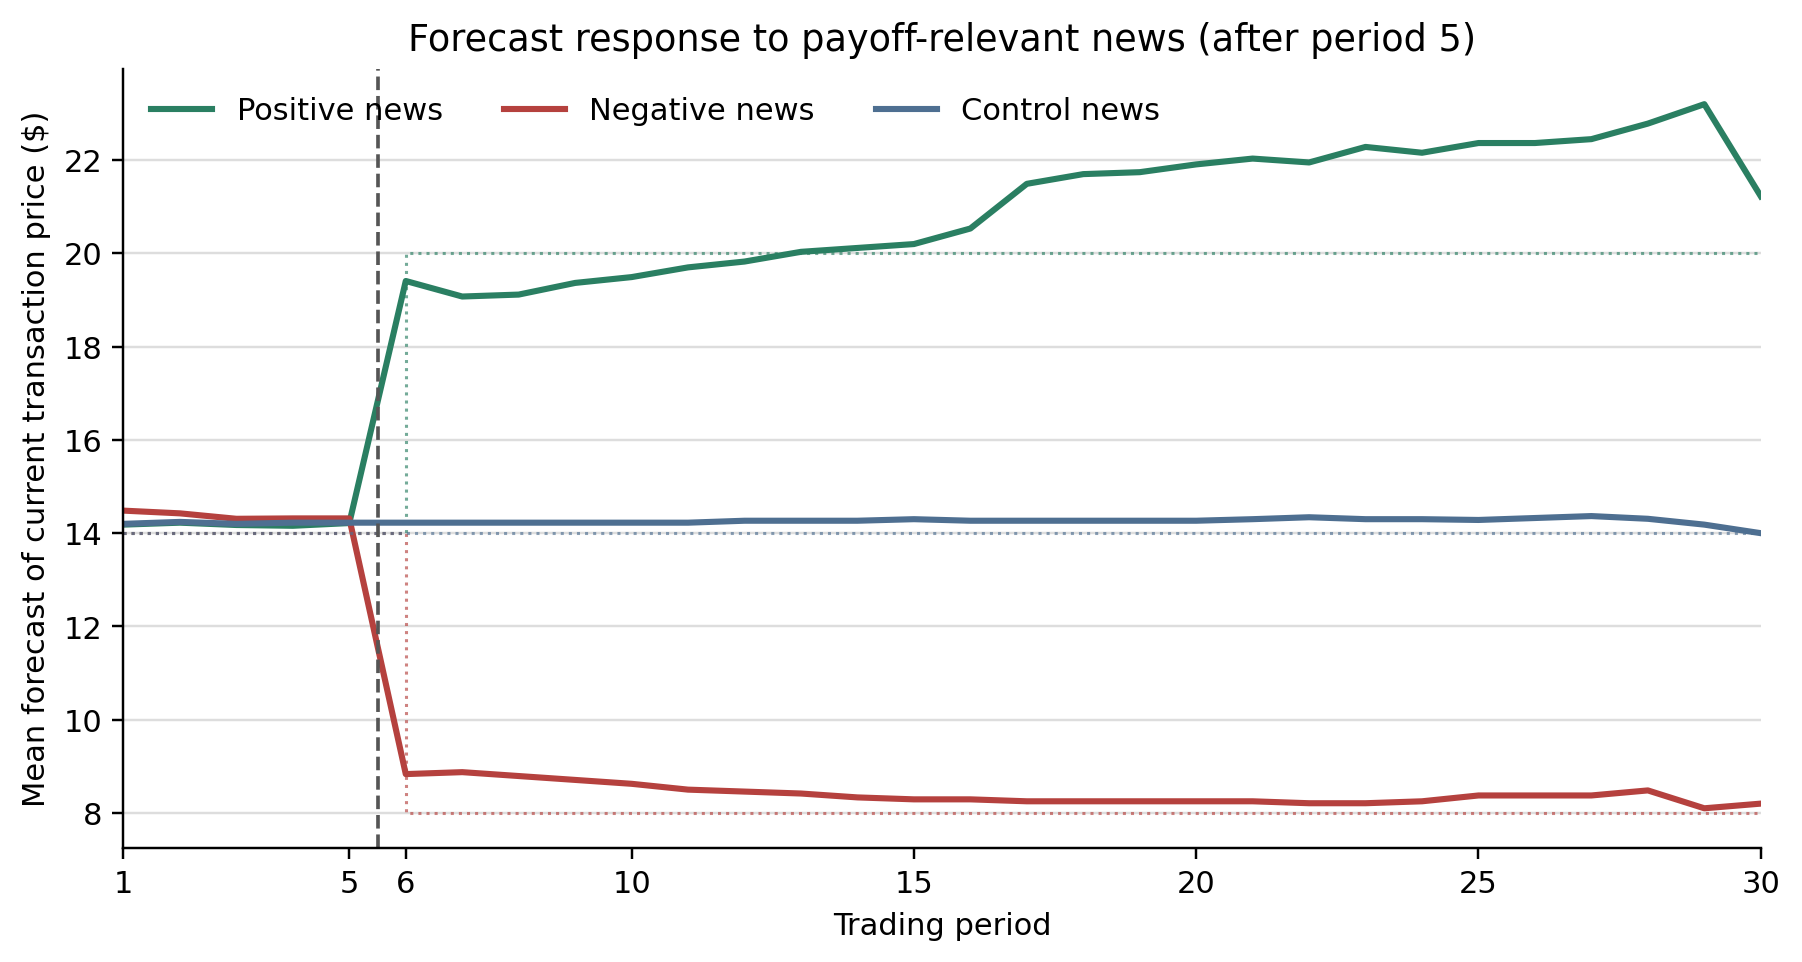
\includegraphics[width=0.91\linewidth]{forecast_paths.png}
\caption{Mean current-price forecasts. Dotted step lines show terminal
redemption: \$14 before the announcement, then the arm-specific value. The
vertical dashed line marks the update between periods 5 and 6.}
\end{figure}

\begin{figure}[ht]
\centering
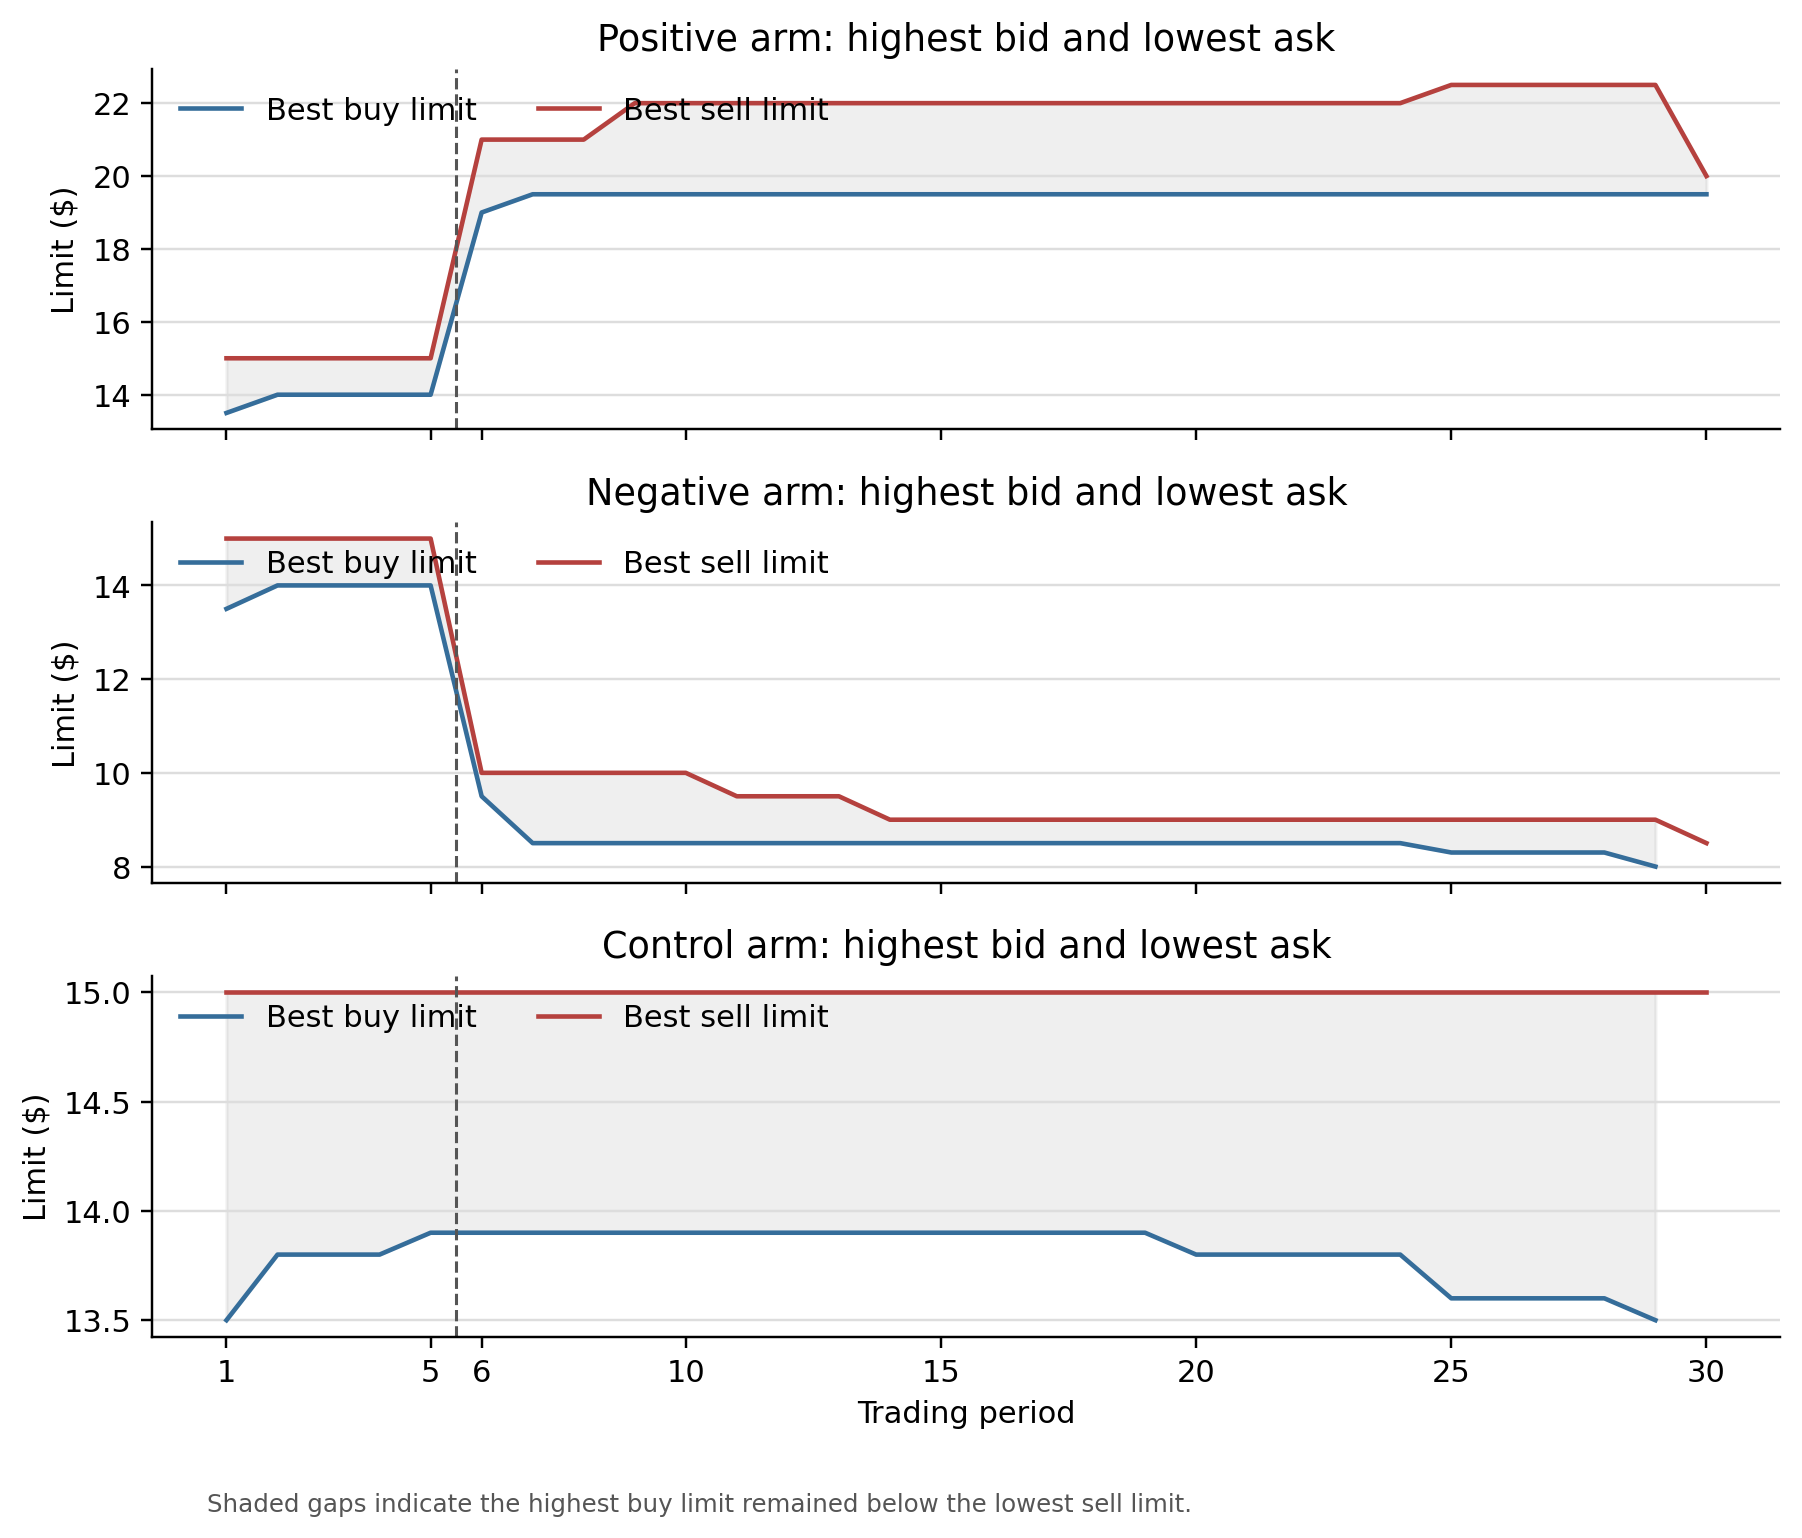
\includegraphics[width=0.91\linewidth]{order_frontiers.png}
\caption{Highest accepted-quantity buy limit and lowest accepted-quantity sell
limit. Shading marks the positive gap between them; no period produced a fill.}
\end{figure}

\begin{figure}[ht]
\centering
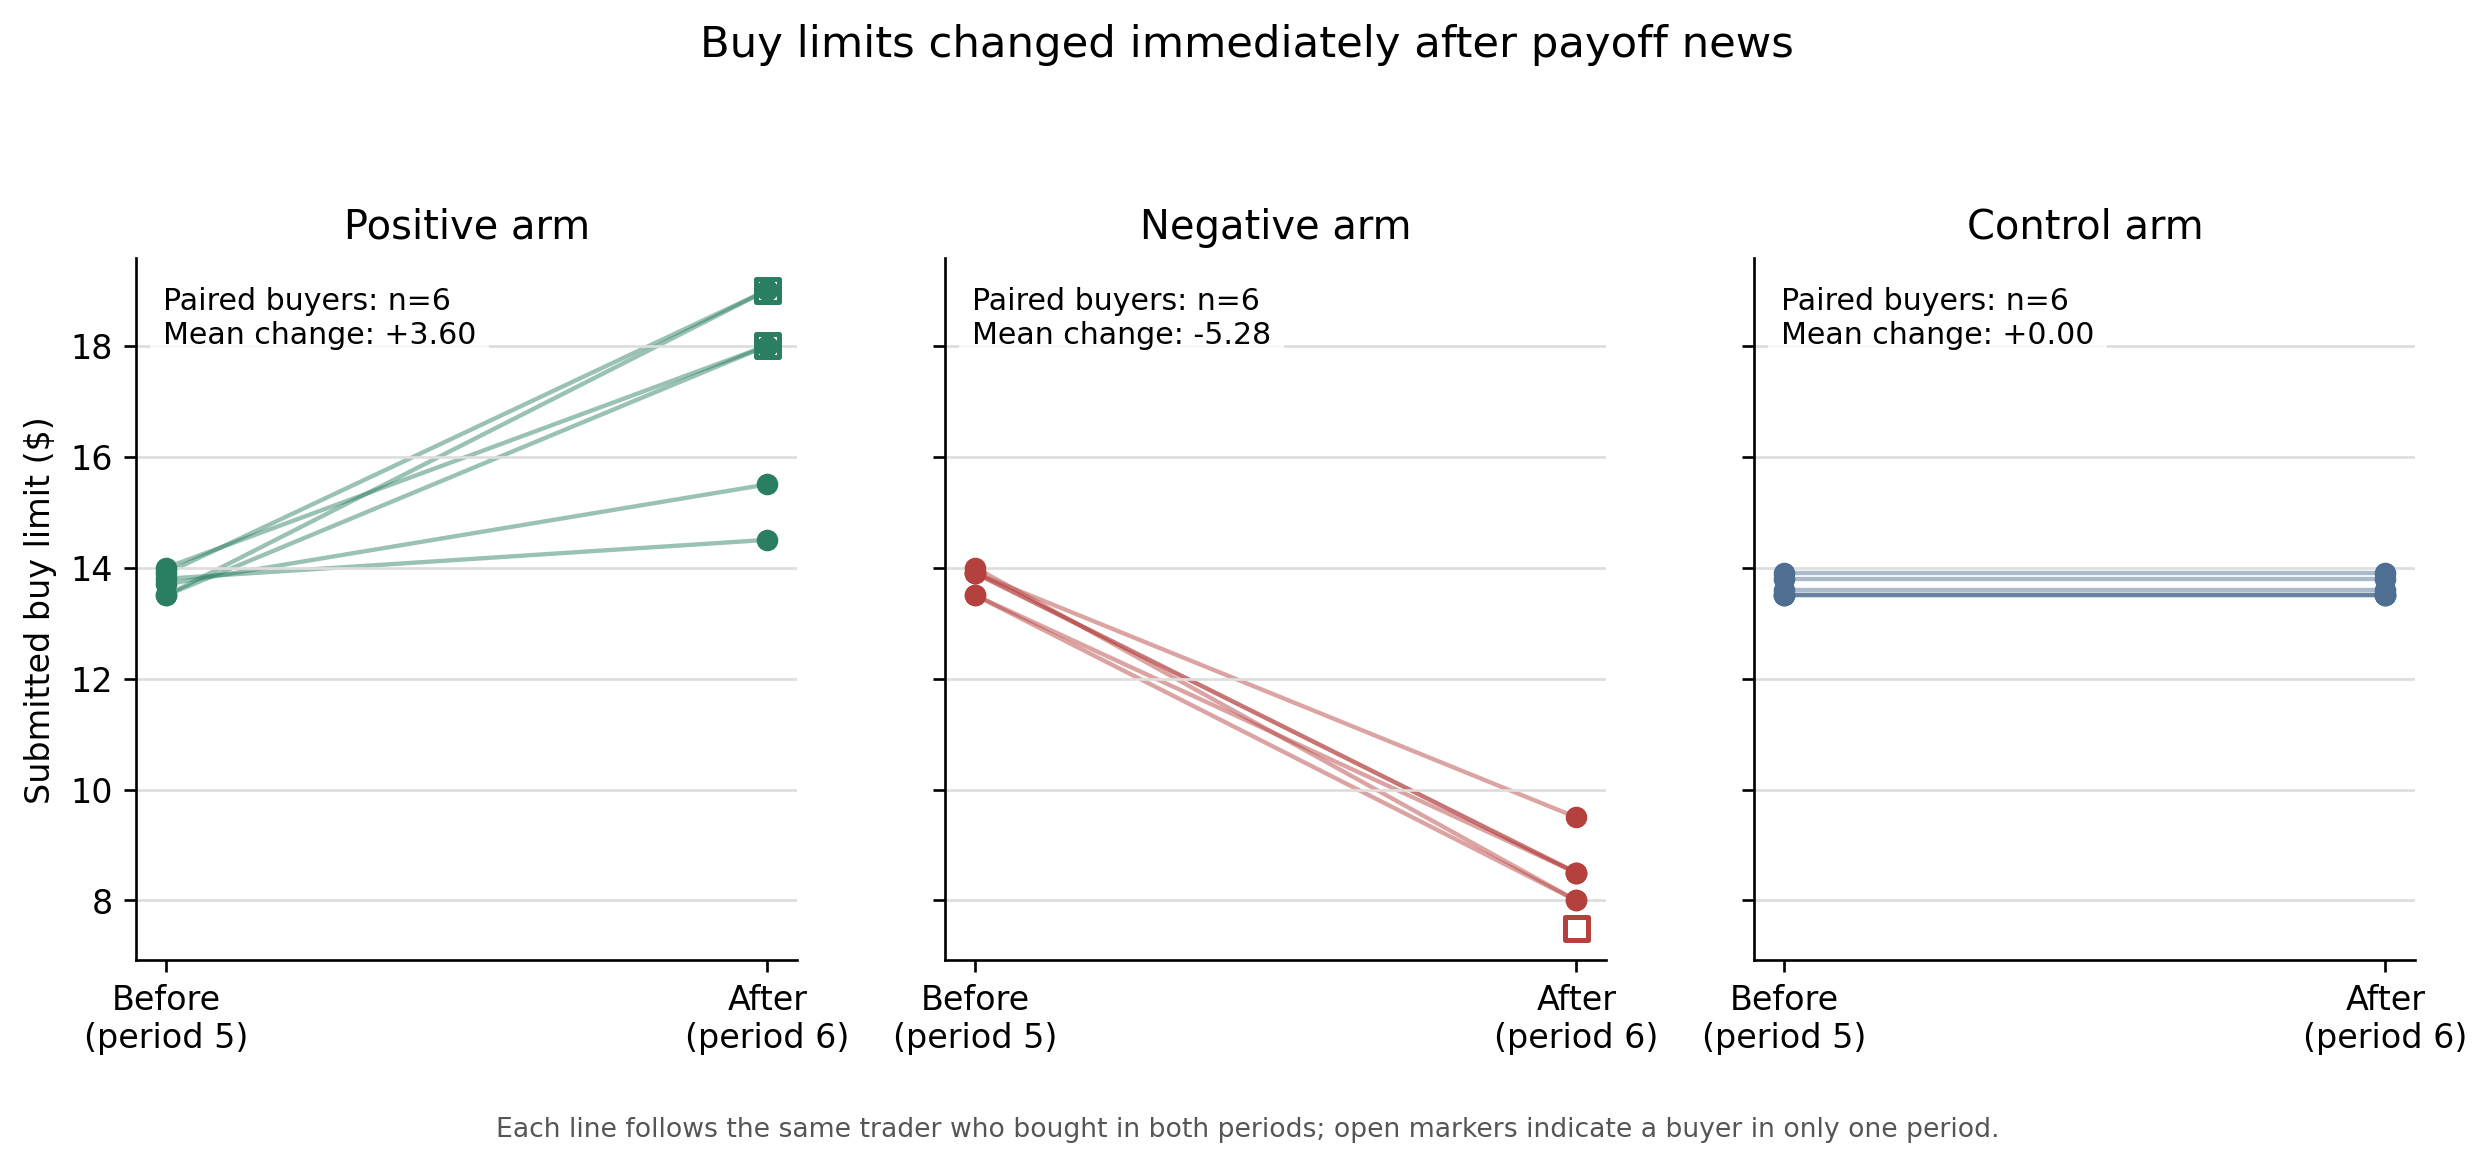
\includegraphics[width=0.96\linewidth]{bids_before_after.png}
\caption{Each line connects one trader's buy limit in period 5 to their limit
in period 6. The positive-news bids move up, negative-news bids move down, and
control bids remain unchanged. Only traders who bought in both periods have a
connecting line; open symbols show a trader who bought in only one period.
There were six paired buyers in each arm.}
\label{fig:bids}
\end{figure}

These are one-market pilots, not treatment-effect estimates. The 12 traders
within a market are not independent experimental units. The next iteration
should keep payoff news and the current machine but prompt both sides to quote
closer to their forecasts using the same pre-specified spread in every arm.
Then run enough independent markets per condition for a market-level power
calculation. This pilot already supports the manipulation check: payoff news
produced large, directionally correct forecast shifts while the no-news control
did not move.

\section{The shared-state machine}
The new \texttt{FundamentalNewsCallMarket} is an EDSL shared-state machine. It
starts from the machine definition returned by EDSL's \texttt{call\_market}
factory, carrying forward its state fields, commands, view, completion rule,
close effects, and native algorithms. The study constructs a new machine of
that same EDSL machine type and extends its definition with live payoff fields
and two commands for announcing and applying the changed redemption. Native
settlement is configured with zero terminal redemption; the new machine applies
the live redemption from state after final income. This avoids a stale
constant being used after a mid-market payoff change. It is a programmatic
extension of the EDSL machine definition, not a Python subclass.

\begin{lstlisting}
base = call_market(TRADERS, rules=machine_rules, seed=seed)
machine = Machine(
    name="FundamentalNewsCallMarket",
    constants=dict(base.constants),
    fields=dict(base.fields),
    commands=dict(base.commands),
    view=dict(base.view),
    algorithms=base.algorithms,
)
machine.fields["terminal_redemption_cents"] = state_field(
    StateType.integer(), 1400
)
machine.fields["fundamental_events"] = state_field(
    StateType.sequence(), []
)
\end{lstlisting}

The machine adds an announcement command that updates the public payoff field
and appends a dated event. Since period-5 settlement advances the machine's
current period to 6, the guard checks for state period 6 even though the event
metadata records delivery after period 5. The event is written before any
period-6 trader reads.

\begin{lstlisting}
machine.commands["announce_payoff_change"] = Command(
    inputs={
        "value_cents": StateType.integer(),
        "message": StateType.text(),
        "period": StateType.integer(),
    },
    require=field("period") == NEWS_PERIOD + 1,
    effects=(
        assign("terminal_redemption_cents", arg("value_cents")),
        assign("announcement", arg("message")),
        append("fundamental_events", record(
            period=arg("period"),
            value_cents=arg("value_cents"),
            message=arg("message"),
        )),
    ),
)
\end{lstlisting}

The read-only participant view exposes the current redemption and announcement
to all traders. In control, no update command executes and the value remains
\$14. Each period otherwise follows the same trader-submit then exchange-settle
sequence.

At period 30, native settlement records each participant's remaining shares
but does not pay redemption. A separate command applies the value from state
over all accounts and sets a one-time guard:

\begin{lstlisting}
accounts_after_redemption = map_items(
    field("accounts"), key="trader", value="account",
    key_expr=local("trader"),
    value_expr=local("account").with_item(
        "cash_cents",
        local("account").get("cash_cents")
        + local("account").get("redeemed_shares")
        * field("terminal_redemption_cents"),
    ),
)
machine.commands["apply_terminal_redemption"] = Command(
    inputs={},
    require=field("finished") & ~field("redemption_applied"),
    effects=(assign("accounts", accounts_after_redemption),
             assign("redemption_applied", True)),
)
\end{lstlisting}

This creates an auditable two-stage end-of-market transition: ordinary income
and account closure first, live terminal payoff second. The detailed diagram
was generated with EDSL's native machine-diagram method.

\begin{figure}[ht]
\centering
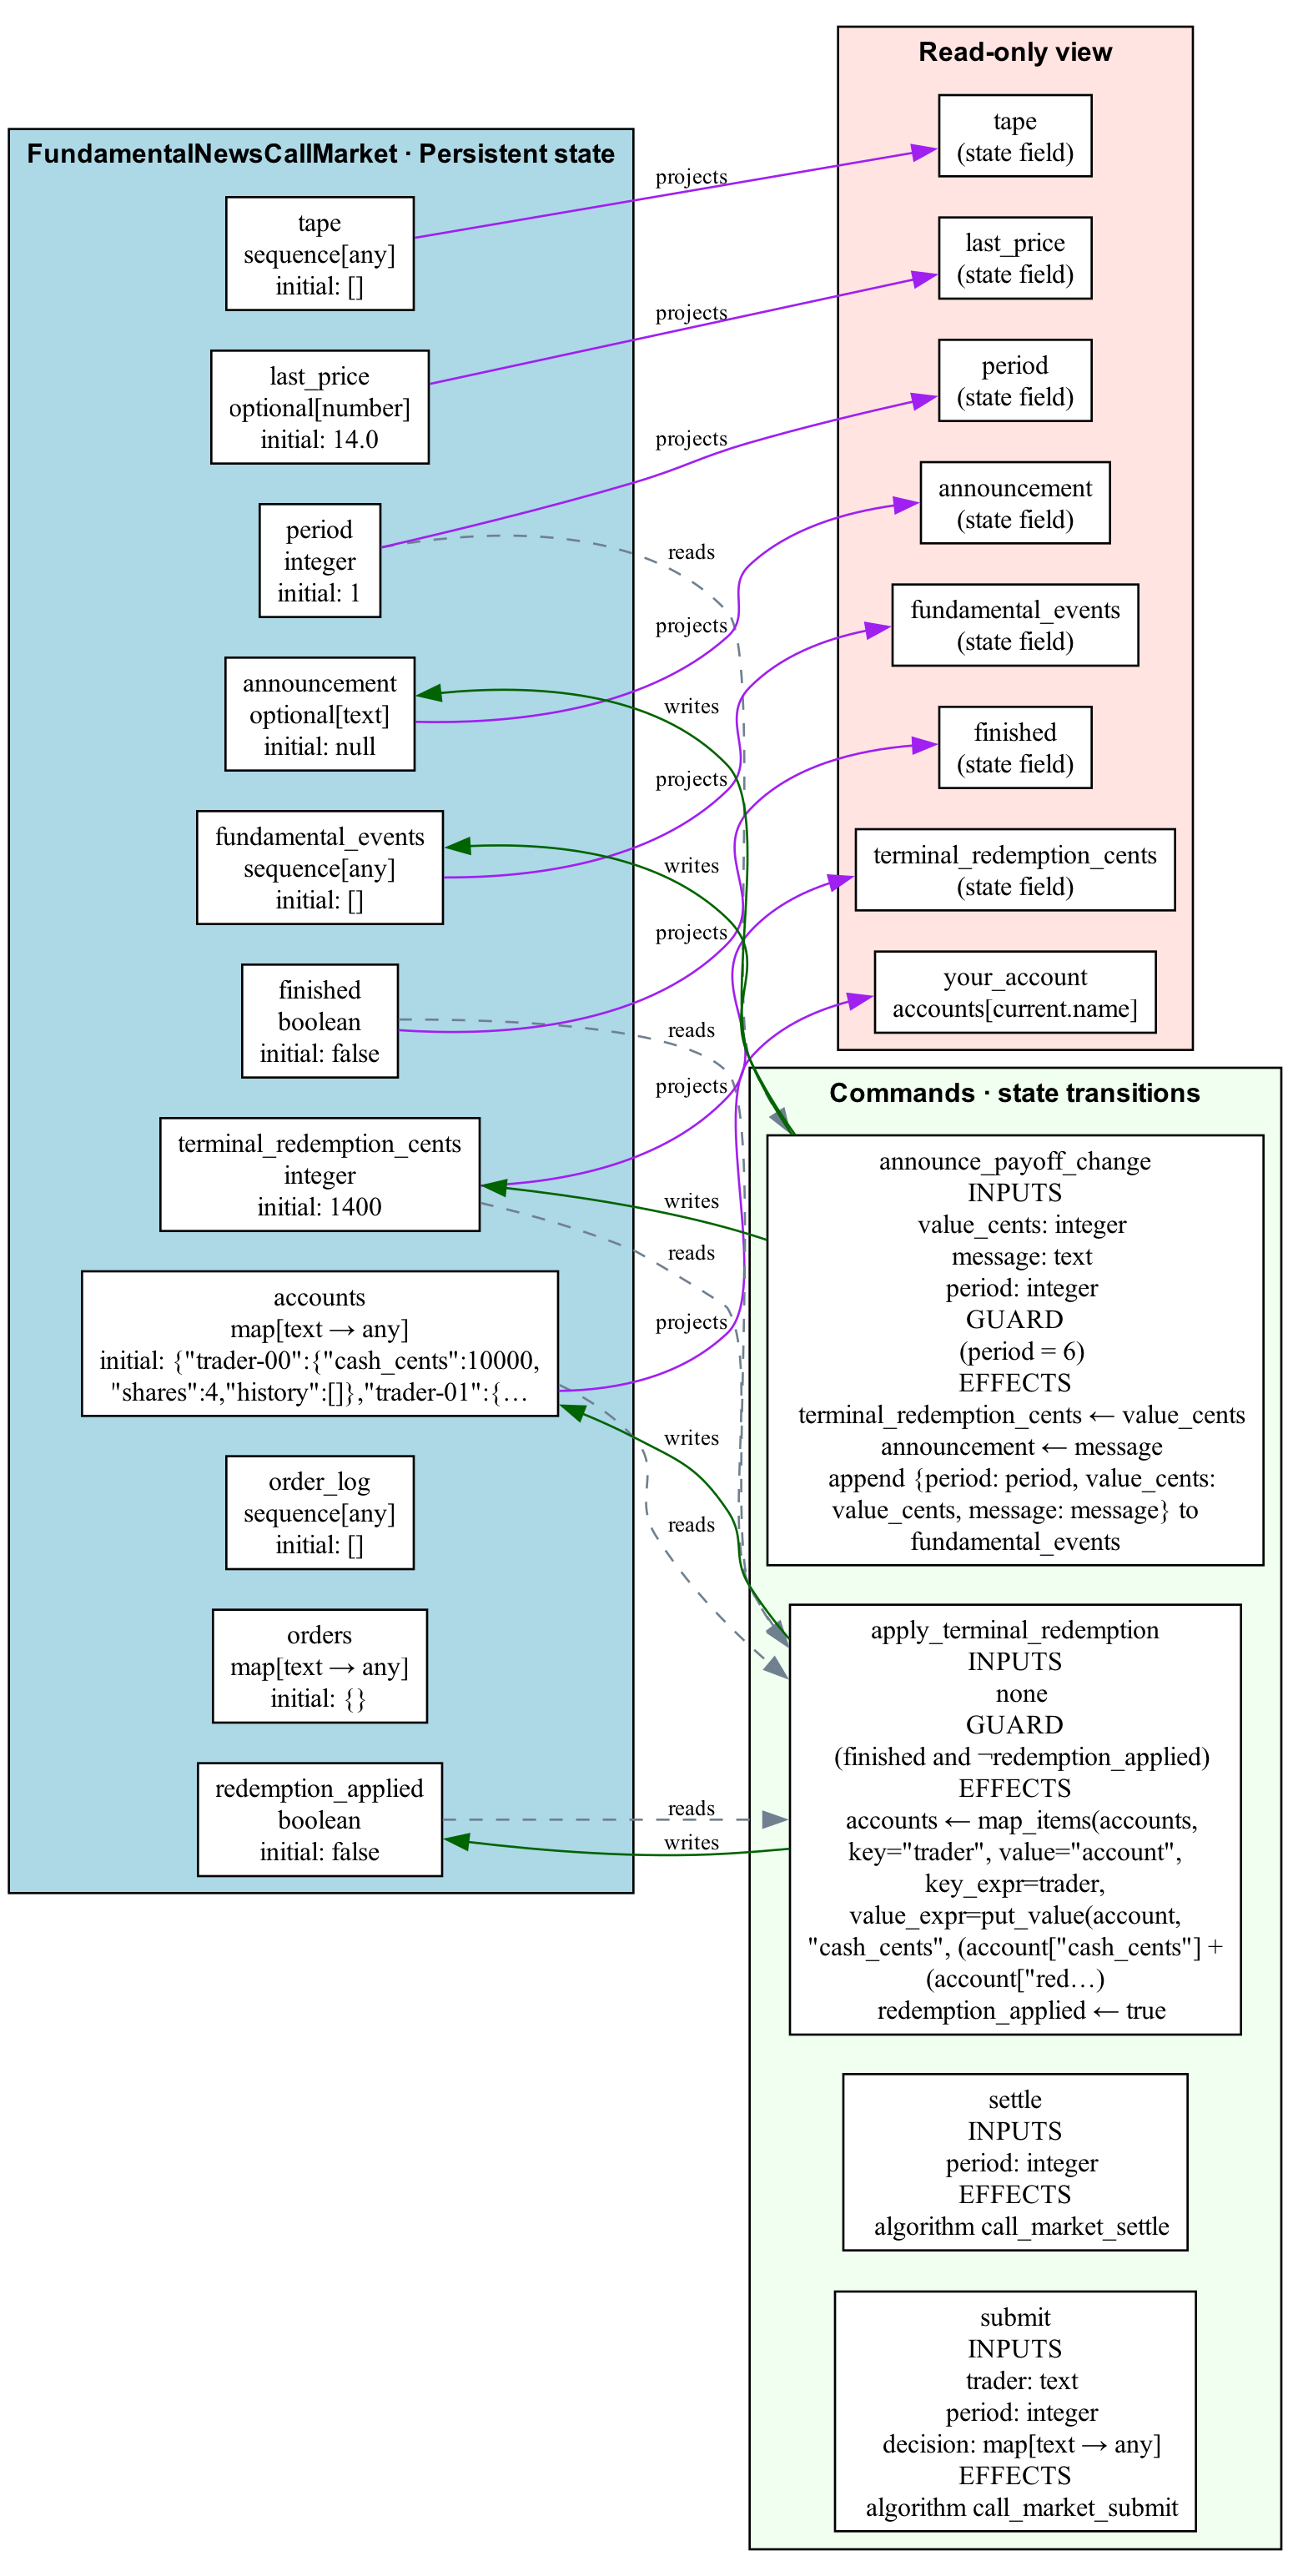
\includegraphics[width=0.67\linewidth,height=0.68\textheight,keepaspectratio]{fundamental_news_machine.png}
\caption{The new market machine: live redemption, public announcement, audit
history, and final payoff command.}
\end{figure}

\section{Execution and audit}
Each corrected arm completed 30 rounds, with 360 trader decisions, 30 native
settlements, and a final redemption command. Positive and negative arms also
completed one scripted payoff-announcement task (392 items each); control
completed 391 items. Final state records confirm redemptions of 2000, 800, and
1400 cents and a successful final payoff application.

The experiment source is \texttt{experiment.py}; serialized specifications,
workflow databases, state event logs, model-call records, and per-arm completion
files are retained beneath \texttt{pilot\_02/}. A first positive run is retained
under \texttt{pilot\_01/} for audit, but excluded: its guard checked period 5
after settlement had advanced state to period 6, so the update was a no-op.
The corrected run used the state-period guard of 6 and recorded an applied
\$20 update.

\end{document}
